\documentclass{article}
\usepackage{amsmath,amsthm}
\usepackage{tikz}

\begin{document}

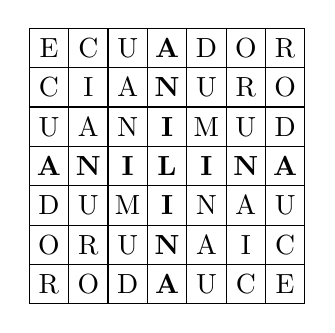
\begin{tikzpicture}
\foreach \x in {1,2,3,4,5,6,7}
\foreach \y in {1,2,3,4,5,6,7}
{
  \draw (\x/2,\y/2)  rectangle ++(0.5,0.5);%+(-1,-1)
}
% words from bottom to top
\draw (0.5,0.5)+(0.25,0.25) node {R};
\draw (1,0.5)+(0.25,0.25) node {O};
\draw (1.5,0.5)+(0.25,0.25) node {D};
\draw (2,0.5)+(0.25,0.25) node {\textbf{A}};
\draw (2.5,0.5)+(0.25,0.25) node {U};
\draw (3,0.5)+(0.25,0.25) node {C};
\draw (3.5,0.5)+(0.25,0.25) node {E};
% -----------------------------------
\draw (0.5,1)+(0.25,0.25) node {O};
\draw (1,1)+(0.25,0.25) node {R};
\draw (1.5,1)+(0.25,0.25) node {U};
\draw (2,1)+(0.25,0.25) node {\textbf{N}};
\draw (2.5,1)+(0.25,0.25) node {A};
\draw (3,1)+(0.25,0.25) node {I};
\draw (3.5,1)+(0.25,0.25) node {C};
% -----------------------------------
\draw (0.5,1.5)+(0.25,0.25) node {D};
\draw (1,1.5)  +(0.25,0.25) node {U};
\draw (1.5,1.5)+(0.25,0.25) node {M};
\draw (2,1.5)  +(0.25,0.25) node {\textbf{I}};
\draw (2.5,1.5)+(0.25,0.25) node {N};
\draw (3,1.5)  +(0.25,0.25) node {A};
\draw (3.5,1.5)+(0.25,0.25) node {U};
% -----------------------------------
\draw (0.5,2)+(0.25,0.25) node {\textbf{A}};
\draw (1,2)  +(0.25,0.25) node {\textbf{N}};
\draw (1.5,2)+(0.25,0.25) node {\textbf{I}};
\draw (2,2)  +(0.25,0.25) node {\textbf{L}};
\draw (2.5,2)+(0.25,0.25) node {\textbf{I}};
\draw (3,2)  +(0.25,0.25) node {\textbf{N}};
\draw (3.5,2)+(0.25,0.25) node {\textbf{A}};
% -----------------------------------
\draw (0.5,2.5)+(0.25,0.25) node {U};
\draw (1,2.5)  +(0.25,0.25) node {A};
\draw (1.5,2.5)+(0.25,0.25) node {N};
\draw (2,2.5)  +(0.25,0.25) node {\textbf{I}};
\draw (2.5,2.5)+(0.25,0.25) node {M};
\draw (3,2.5)  +(0.25,0.25) node {U};
\draw (3.5,2.5)  +(0.25,0.25) node{D};
% -----------------------------------
\draw (0.5,3)+(0.25,0.25) node {C};
\draw (1,3)  +(0.25,0.25) node {I};
\draw (1.5,3)+(0.25,0.25) node {A};
\draw (2,3)  +(0.25,0.25) node {\textbf{N}};
\draw (2.5,3)+(0.25,0.25) node {U};
\draw (3,3)  +(0.25,0.25) node {R};
\draw (3.5,3)  +(0.25,0.25) node{O};
% -----------------------------------
\draw (0.5,3.5)+(0.25,0.25) node {E};
\draw (1,3.5)  +(0.25,0.25) node {C};
\draw (1.5,3.5)+(0.25,0.25) node {U};
\draw (2,3.5)  +(0.25,0.25) node {\textbf{A}};
\draw (2.5,3.5)+(0.25,0.25) node {D};
\draw (3,3.5)  +(0.25,0.25) node {O};
\draw (3.5,3.5)  +(0.25,0.25) node{R};
\end{tikzpicture}

\end{document}